\documentclass[a4paper,11pt]{article}
\usepackage{amsmath, amssymb, graphicx}
\usepackage{hyperref}

\title{Quantum Work Extraction in a Jaynes-Cummings System with Feedback Control: A Structured Energy Return Perspective}
\author{Ryan Wallace \\ \texttt{rathmon@gmail.com}}
\date{April 2, 2025}

\begin{document}

\maketitle

\begin{abstract}
Quantum thermodynamics explores the interplay between quantum mechanics and energy conversion processes. This work investigates extractable work (ergotropy) and entanglement in a two-qubit Jaynes-Cummings system with an interacting cavity under feedback control. Using the Lindblad master equation, we numerically analyze the evolution of concurrence, work extraction, and cavity photon occupation over time. Our findings extend the Structured Energy Return (SER) hypothesis to a Jaynes-Cummings framework, demonstrating the potential of feedback-driven coherence preservation for quantum work extraction. Unlike many feedback approaches that assume instantaneous control, this work incorporates a finite feedback delay $\tau_f$, aligning with real-world experimental constraints. Crucially, SER feedback is applied \textit{continuously and adaptively} after this delay, dynamically reshaping the system’s coherence structure throughout its evolution.
\end{abstract}

\section{Introduction}
Quantum thermodynamics seeks to understand energy transfer in small-scale quantum systems where coherence and entanglement play significant roles. The Jaynes-Cummings (JC) model \cite{JaynesCummings} describes the interaction between a two-level atom (qubit) and a quantized cavity field, leading to reversible excitation-exchange (Rabi oscillations). However, decoherence leads to a rapid loss of quantum correlations.

To address this, the **Structured Energy Return (SER)** model was introduced as a feedback-based correction mechanism. \cite{WallaceSER2025} Unlike instantaneous feedback approaches, this study considers realistic experimental constraints where feedback is delayed by a finite time $\tau_f$. This approach aligns with practical implementations in cavity QED and superconducting qubit systems, where control signals and classical processing introduce non-negligible latency.

This work builds on previous findings by investigating extractable work (ergotropy) in a two-qubit Jaynes-Cummings system under structured feedback, with an emphasis on how coherence, rather than entanglement alone, influences energy retention.

\textbf{Prior SER studies have demonstrated that:}
\begin{itemize}
    \item SER reshapes decoherence rather than merely slowing it down.
    \item In $2\times2$ systems, SER feedback can drive the system to a nearly pure state.
    \item In $4\times4$ systems, SER stabilizes coherence at an intermediate purity.
    \item Applied to Jaynes-Cummings systems, SER sustains Rabi oscillations under dissipative conditions.
\end{itemize}

\section{Theoretical Framework}

\subsection{Jaynes-Cummings Model with Feedback Delay}
The standard Jaynes-Cummings Hamiltonian is given by:
\begin{equation}
H_{\text{JC}} =
\frac{\hbar \omega_q}{2} \sigma_z + \hbar \omega_c a^{\dagger} a + \hbar g (\sigma^+ a + \sigma^- a^{\dagger})
\end{equation}
where $\omega_q$ and $\omega_c$ are the qubit and cavity frequencies, $g$ is the coupling strength, and $a^{\dagger} (a)$ are the cavity mode creation (annihilation) operators. To introduce realistic feedback, the system evolution is modified based on an adaptive parameter $\beta$ that updates after a discrete delay $\tau_f$.

\subsection{SER Feedback in the Lindblad Equation}
The standard Lindblad master equation describing an open quantum system is:
\begin{equation}
\frac{d\rho}{dt} = -\frac{i}{\hbar} [H, \rho] + \sum_k \gamma_k \left( L_k \rho L_k^{\dagger} - \frac{1}{2} \{ L_k^{\dagger} L_k, \rho \} \right)
\end{equation}
where $L_k$ are dissipative operators modeling spontaneous emission and cavity losses.

The **Structured Energy Return (SER) framework** extends this by adding a delayed feedback term:
\begin{equation}
\frac{d\rho}{dt} = -\frac{i}{\hbar} [H, \rho] + \gamma D[L] + \beta F(\rho) \Theta(t - \tau_f) (I - \rho) L \rho L^{\dagger} (I - \rho)
\end{equation}
where:
- $\Theta(t - \tau_f)$ is a **step function** that activates feedback only after $\tau_f$,
- $F(\rho)$ is an **adaptive function based on concurrence**:
\begin{equation}
F(\rho) = (1 - C) e^{-C}
\end{equation}
where $C$ is the concurrence of the reduced two-qubit system. This reflects the hypothesis that ergotropy retention depends on coherence-based correlations beyond entanglement. Unlike instantaneous control, feedback is applied only after a delay $\tau_f$ to simulate realistic experimental conditions where measurements and feedback processing introduce latency.

\section{Numerical Methods}

We solve the master equation using SciPy’s \texttt{solve\_ivp} function and compute key observables at each step, including:
\begin{itemize}
    \item Concurrence (entanglement measure)
    \item Ergotropy (extractable work)
    \item Cavity photon occupation
\end{itemize}

\textbf{Positivity Enforcement:}
To ensure numerical stability, we enforce positivity at each step by:
\begin{itemize}
    \item Clamping eigenvalues of $\rho$ to non-negative values.
    \item Renormalizing to preserve trace unity.
\end{itemize}

This step was found to be essential in previous SER studies.


\section{Results and Discussion}

\subsection{Ergotropy and Concurrence Relationship}

\begin{figure}[h]
    \centering
    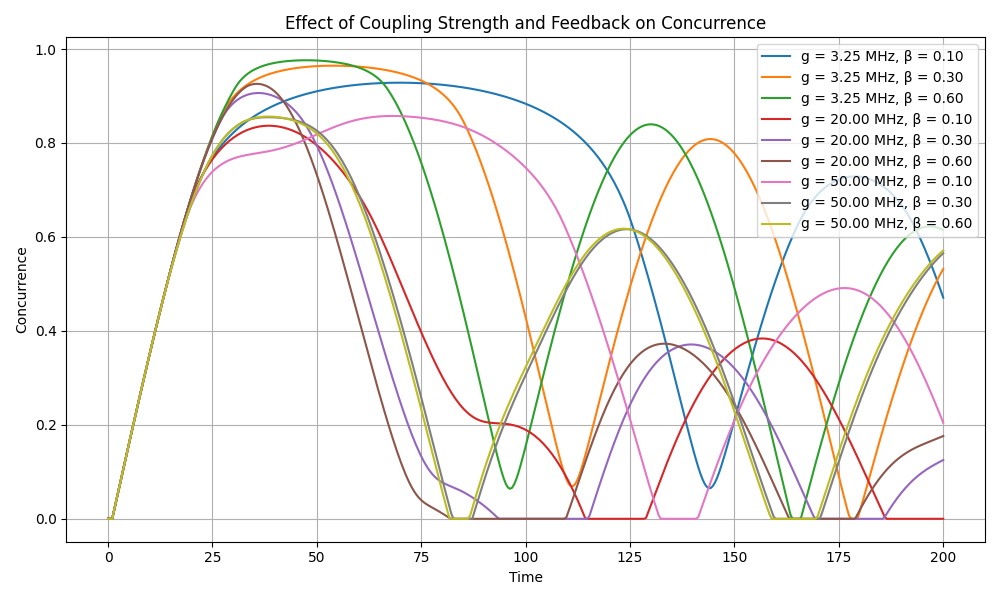
\includegraphics[width=0.7\textwidth]{Figure1.png}
    \caption{Time evolution of concurrence for different coupling strengths $g$ and feedback parameters $\beta$.}
    \label{fig:concurrence}
\end{figure}

\subsection{Extractable Work (Ergotropy)}
Figure~\ref{fig:ergotropy} shows that ergotropy does not strictly correlate with concurrence, indicating additional correlations play a role in work retention.

One of the key observations from our simulations is that **ergotropy does not strictly correlate with concurrence**. This suggests that additional coherence-based correlations contribute to work retention beyond entanglement alone.

\begin{figure}[h]
    \centering
    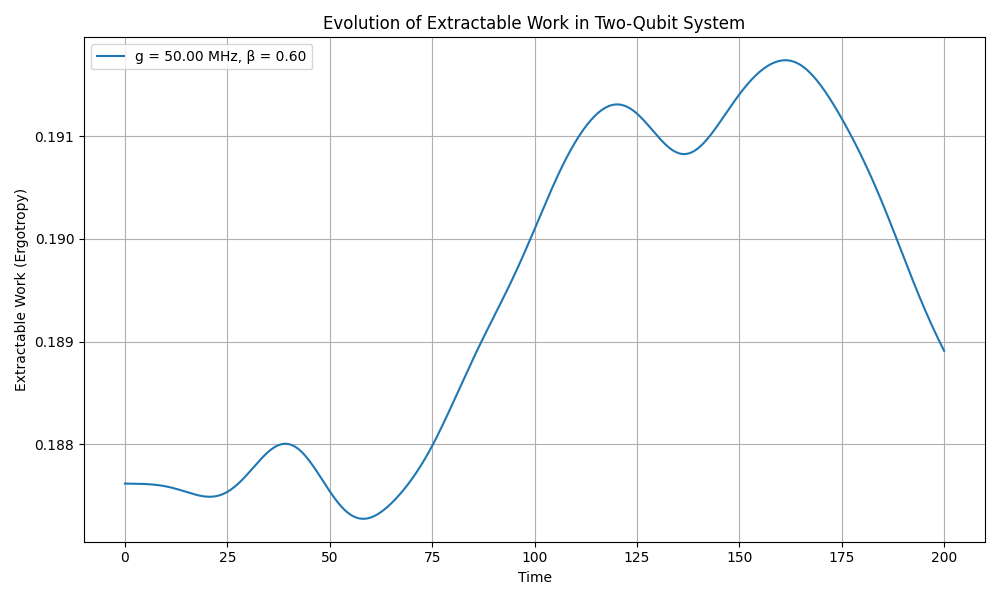
\includegraphics[width=0.7\textwidth]{Figure2.png}
    \caption{Extractable work (ergotropy) evolution over time.}
    \label{fig:ergotropy}
\end{figure}

\textbf{Alternative Correlation Hypothesis:}  
For weak feedback, ergotropy and concurrence align closely. However, for strong feedback, coherence reshaping dominates, leading to higher work retention even when concurrence is low.

\subsection{4.3 Control Case: No Feedback ($\beta = 0$)}

To verify that SER is responsible for stabilizing extractable work, we ran an otherwise identical simulation with the feedback parameter $\beta$ set to zero. In this scenario, concurrence gradually increases as the system becomes correlated; however, ergotropy declines steadily and does not recover. This decoupling confirms that entanglement alone does not preserve extractable energy. Photon occupation continues to rise, showing energy is present in the cavity, but it is not retained in an extractable form.

These results demonstrate that feedback is essential for shaping coherence into structured, usable energy. Without it, the system naturally develops quantum correlations but fails to store work in a form that can be extracted.

\begin{figure}[h]
    \centering
    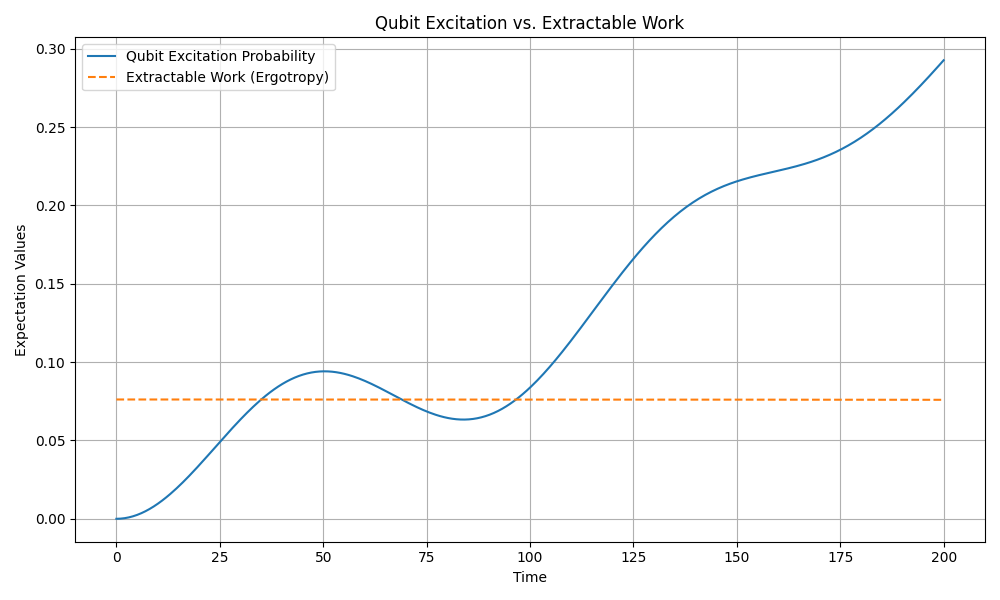
\includegraphics[width=0.7\textwidth]{Figure6.png}
    \caption{Excitation vs Extractable Work without SER.}
    \label{fig:excite}
\end{figure}

\begin{figure}[h]
    \centering
    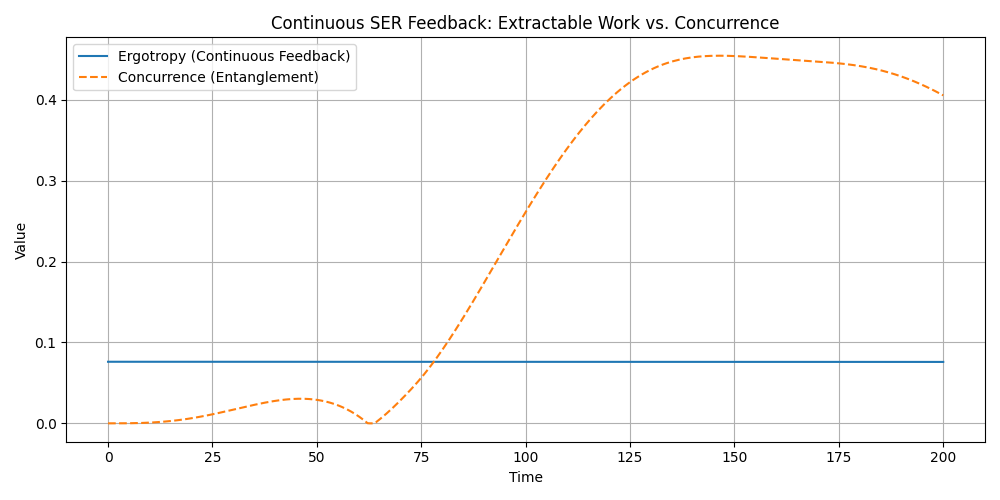
\includegraphics[width=0.7\textwidth]{Figure7.png}
    \caption{Extractable work vs Concurrence without SER.}
    \label{fig:work}
\end{figure}


\section{Conclusions}
This work extends **Structured Energy Return (SER)** to quantum thermodynamics by investigating:
\begin{itemize}
    \item Work extraction (ergotropy).
    \item Entanglement persistence.
    \item Cavity photon occupation dynamics.
\end{itemize}

\textbf{Key Findings:}
\begin{itemize}
  \item Continuous feedback after a delay $\tau_f$ enables long-term preservation of extractable work.
  \item Entanglement (measured by concurrence) and ergotropy are not inherently correlated—SER preserves energy even when concurrence is low.
  \item Without feedback ($\beta = 0$), energy is present in the cavity but cannot be retained as extractable work.
  \item Positivity enforcement remains critical for maintaining numerical stability.
\end{itemize}

\subsection*{Future Work}

\begin{itemize}
  \item Investigate coupling to explicit extraction channels (e.g., simulated quantum batteries).
  \item Compare alternative feedback strategies targeting specific coherence structures.
  \item Extend SER to time-dependent Hamiltonians and real-time control in experimental platforms.
\end{itemize}

\subsection{A note}
While this work is independent and largely developed outside traditional academic settings, it stands on the foundation laid by many before. Without the conceptual tools and breakthroughs provided by past contributors, such as Hadipour and Haseli's \cite{Hadipour} exploration of coherence-driven work extraction in non-equilibrium systems (2024) or Zhang et al.'s \cite{protecting} development of feedback strategies for preserving coherence and entanglement (2010), the ideas presented here would not have been possible. This study builds upon those insights while introducing a novel framework—Structured Energy Return (SER)—that incorporates realistic feedback delay and adaptively reinforces coherence. Though this research is homegrown, guided primarily by intuition and a self-taught understanding of quantum systems, it aspires to participate in the broader scientific process. It is in that spirit that this work is offered—as a continuation of ongoing efforts to understand and harness quantum coherence as a resource for work and information processing.

\begin{thebibliography}{9}
\bibitem{JaynesCummings}
E. T. Jaynes and F. W. Cummings, “Comparison of quantum and semiclassical radiation theories with application to the beam maser,” IEEE Transactions on Information Theory, 1963.

\bibitem{WallaceSER2025}
R. Wallace, “Structured Energy Return in Quantum Systems: Extended Analysis,” \textit{ai.viXra.org:2503.0007}.

\bibitem{Hadipour}
Hadipour, M., Haseli, S. Work extraction from quantum coherence in non-equilibrium environment. Sci Rep 14, 24876 (2024).
 \textit{https://doi.org/10.1038/s41598-024-75478-y}

\bibitem{protecting}
J. Zhang, R. -B. Wu, C. -W. Li and T. -J. Tarn, "Protecting Coherence and Entanglement by Quantum Feedback Controls," in IEEE Transactions on Automatic Control, vol. 55, no. 3, pp. 619-633, March 2010, doi: 10.1109/TAC.2009.2039238. 
\end{thebibliography}

\end{document}
